%%%%%%%%%%%%%%%%%%%%%%%%%%%%%%%%%%%%%%%%%%%%%%%%%%%%%%%%%%%%%%%%%%%%%%%%%%%%%%%%
% \documentclass[t]{beamer}
\usepackage[
    orientation=landscape,
    size=custom,
    width=25.4,
    height=19.05,
    scale=0.63 % erzeugt 16pt Schriftgröße
]{beamerposter}

\newcommand{\PraesentationSchriftgroesseSehrGross}{\fontsize{30}{45}}
\newcommand{\PraesentationSchriftgroesseGross}{\fontsize{22}{33}}
\newcommand{\PraesentationSchriftgroesseNormal}{\fontsize{16}{29}}
\newcommand{\PraesentationSchriftgroesseKlein}{\fontsize{12}{18}}
\newcommand{\PraesentationSchriftgroesseDreizeiler}{\fontsize{7}{10}}
\newcommand{\PraesentationSchriftgroesseAufzaehlungszeichen}{\fontsize{10}{8}}

\newcommand{\PraesentationAbstandAbsatz}{22.1pt}
\newcommand{\PraesentationPositionKorrekturOben}{0cm}
\newcommand{\PraesentationBeispieleSchriftgroessen}{30 | 22 | 16 | 12}
\input{./Ressourcen/Praesentation/Praeambel.tex} % Layout 4:3
%\documentclass[aspectratio=169]{beamer}
\documentclass[t,aspectratio=169]{beamer}
\usepackage[
    orientation=landscape,
    size=custom,
    width=25.4,
    height=14.2875,
    scale=0.5
]{beamerposter}

\newcommand{\PraesentationSchriftgroesseSehrGross}{\fontsize{25}{38}}
\newcommand{\PraesentationSchriftgroesseGross}{\fontsize{18}{27}}
\newcommand{\PraesentationSchriftgroesseNormal}{\fontsize{14}{21}}
\newcommand{\PraesentationSchriftgroesseKlein}{\fontsize{11}{17}}
\newcommand{\PraesentationSchriftgroesseDreizeiler}{\fontsize{7}{10}}
\newcommand{\PraesentationSchriftgroesseAufzaehlungszeichen}{\fontsize{10}{8}}

\newcommand{\PraesentationAbstandAbsatz}{18pt}
\newcommand{\PraesentationPositionKorrekturOben}{-1cm}
\newcommand{\PraesentationBeispieleSchriftgroessen}{25 | 18 | 14 | 11}
\usepackage[utf8]{inputenc}
\usepackage[T1]{fontenc} % Zeichensatzkodierung

\usepackage{calc} % Berechnungen

\usepackage{relsize}
\usepackage{xspace}
\usepackage{listings}

%\usepackage[ngerman]{babel} % Deutsche Lokalisierung
\usepackage{graphicx} % Grafiken
\graphicspath{ {./Assets/} }
\usepackage{caption,setspace}
\usepackage[export]{adjustbox}
\usepackage[absolute, overlay]{textpos} % Positionierung
% Silbentrennung:
\usepackage{hyphenat}
%\tolerance 2414
%\hbadness 2414
%\emergencystretch 1.5em
%\hfuzz 0.3pt
%\widowpenalty=10000     % Hurenkinder
%\clubpenalty=10000      % Schusterjungen
%\vfuzz \hfuzz

% Euro-Symbol:
\usepackage[gen]{eurosym}
\DeclareUnicodeCharacter{20AC}{\euro{}}

% Schriftart Helvetica:
\usepackage[scaled]{helvet}
\renewcommand{\familydefault}{\sfdefault}

\usepackage{mathptmx} % skalierbare Formelschriften

\usepackage{tabularx}

\usepackage{multicol} % mehrspaltiger Text


\usepackage{tikz}
\usetikzlibrary{arrows.meta,decorations.markings,calc,shapes.geometric,shadows,arrows}
\usepackage{pgfplots}
\usepackage{pgfplotstable}


\usepackage{amsmath}
\usepackage{amssymb}
\usepackage{amsfonts}
\usepackage{amsthm}
\newtheorem*{thm}{Theorem}
\newtheorem*{dfn}{Definition}
\newtheorem*{lma}{Lemma}

\usepackage{colonequals}

\DeclareMathAlphabet{\mathcal}{OMS}{cmsy}{m}{n}

\newcommand*{\logeq}{\ratio\Leftrightarrow}

% Erweiterbare Fusszeile:
\newcommand{\PraesentationFusszeileZusatz}{}

% Define TUM corporate design colors
% Taken from http://portal.mytum.de/corporatedesign/index_print/vorlagen/index_farben
\definecolor{TUMBlue}{HTML}{0065BD}
\definecolor{TUMSecondaryBlue}{HTML}{005293}
\definecolor{TUMSecondaryBlue2}{HTML}{003359}
\definecolor{TUMBlack}{HTML}{000000}
\definecolor{TUMWhite}{HTML}{FFFFFF}
\definecolor{TUMDarkGray}{HTML}{333333}
\definecolor{TUMGray}{HTML}{808080}
\definecolor{TUMLightGray}{HTML}{CCCCC6}
\definecolor{TUMAccentGray}{HTML}{DAD7CB}
\definecolor{TUMAccentOrange}{HTML}{E37222}
\definecolor{TUMAccentGreen}{HTML}{A2AD00}
\definecolor{TUMAccentLightBlue}{HTML}{98C6EA}
\definecolor{TUMAccentBlue}{HTML}{64A0C8}


\newcommand{\LL}{\mathcal{L}}
\newcommand{\RR}{\mathcal{R}}
\newcommand{\repof}{\mathrm{rep\_of}_\mathcal{L}\,}
\newcommand{\ufabstart}{\mathrm{ufa\_}\beta\mathrm{\_start}_\mathcal{L}}
\newcommand{\ufabtrans}{\mathrm{ufa\_}\beta^+_\mathcal{L}}
\newcommand{\ufabrefl}{\mathrm{ufa\_}\beta^*_\mathcal{L}}
\newcommand{\ufaalpha}{\mathrm{ufa\_}\alpha_\mathcal{L}}
\newcommand{\level}{\mathrm{level}_{\LL,\RR}\,}
\newcommand{\iindex}{\mathrm{index}_{\LL,\RR}\,}
\newcommand{\philr}{\phi\, \LL\, \RR\,}
\newcommand{\philrb}{\phi\, \LL\, \RR}
\newcommand{\Philr}{\Phi\, \LL\, \RR\,}
\newcommand{\Philrb}{\Phi\, \LL\, \RR}
\newcommand{\ufaunion}{\mathrm{ufa\_union}_\LL\,}
\newcommand{\ufaunionl}{\mathrm{union\_by\_rank^{(\LL)}_{\LL,\RR}}\,}
\newcommand{\ufaunionrkl}{\mathrm{union\_by\_rank^{(\RR)}_{\LL,\RR}}\,}
\newcommand{\toppart}{\mathrm{top\_part}_{\LL,\RR}\,}
\newcommand{\pleasant}{\mathrm{pleasant}_{\LL,\RR}\,}
\newcommand{\displeasure}{\mathrm{displeasure}_{\LL,\RR}\,}




 % Layout 16:9
%%%%%%%%%%%%%%%%%%%%%%%%%%%%%%%%%%%%%%%%%%%%%%%%%%%%%%%%%%%%%%%%%%%%%%%%%%%%%%%%


%%%%%%%%%%%%%%%%%%%%%%%%%%%%%%%%%%%%%%%%%%%%%%%%%%%%%%%%%%%%%%%%%%%%%%%%%%%%%%%%
% Für die Person anpassen:

\newcommand{\PersonTitel}{}
\newcommand{\PersonVorname}{Adrián}
\newcommand{\PersonNachname}{Löwenberg Casas}
\newcommand{\PersonStadt}{Munich}
\newcommand{\PersonAdresse}{%
   % @Adresse@\\%
   % @Plz@~\PersonStadt%
}
\newcommand{\PersonTelefon}{%@Telefon@
}
\newcommand{\PersonFax}{%@Fax@
}
\newcommand{\PersonEmail}{adrian.loewenberg@tum.de}
\newcommand{\PersonWebseite}{in.tum.de/~casasa}

\newcommand{\FakultaetAnsprechpartner}{%@Ansprechpartner@
}
% Fakultät:
\newcommand{\FakultaetName}{Department of Informatics}
\newcommand{\LehrstuhlName}{Chair for Logic and Verification}


\hyphenation{} % eigene Silbentrennung
                    
%%%%%%%%%%%%%%%%%%%%%%%%%%%%%%%%%%%%%%%%%%%%%%%%%%%%%%%%%%%%%%%%%%%%%%%%%%%%%%%%

\newcommand{\Rplus}{\protect\hspace{-.1em}\protect\raisebox{.35ex}{\smaller{\smaller\textbf{+}}}}
\newcommand{\Cpp}{\mbox{C\Rplus\Rplus}\xspace}
\newcommand{\CppTw}{\mbox{C\Rplus\Rplus 20}\xspace}

\newcommand{\Datum}{\today}

\renewcommand{\PraesentationFusszeileZusatz}{| Amortized Time Complexity of Union-Find in Isabelle/HOL}

\title{Amortized Time Complexity of Union-Find in Isabelle/HOL \newline \newline {\Large Colloquium to the Bachelor's Thesis \newline}}
\author{\PersonTitel{} \PersonVorname{} \PersonNachname}
\institute[]{\UniversitaetName \\ \FakultaetName \\ \LehrstuhlName {\newline}
Supervisor: Prof. Tobias Nipkow, Ph.D. {\newline} Advisor: Maximilian P.L. Haslbeck, M.Sc.}
\date[\Datum]{\PersonStadt, October 16, 2019}
\subject{Amortized Time Complexity of Union-Find in Isabelle/HOL}


%%%%%%%%%%%%%%%%%%%%%%%%%%%%%%%%%%%%%%%%%%%%%%%%%%%%%%%%%%%%%%%%%%%%%%%%%%%%%%%%
%%%%%%%%%%%%%%%%%%%%%%%%%%%%%%%%%%%%%%%%%%%%%%%%%%%%%%%%%%%%%%%%%%%%%%%%%%%%%%%%
% EINSTELLUNGEN
%%%%%%%%%%%%%%%%%%%%%%%%%%%%%%%%%%%%%%%%%%%%%%%%%%%%%%%%%%%%%%%%%%%%%%%%%%%%%%%%

% Allgemein:
\newcommand{\AllgemeinGestalter}{ediundsepp Gestaltungsgesellschaft}
\newcommand{\AllgemeinErsteller}{eWorks GmbH}

% Universität:
\newcommand{\UniversitaetName}{Technische Universität München}
\newcommand{\UniversitaetAbkuerzung}{TUM}
\newcommand{\UniversitaetWebseite}{www.tum.de}
\newcommand{\UniversitaetLogoBreite}{19mm}
\newcommand{\UniversitaetLogoHoehe}{1cm}

\newcommand{\UniversitaetAdresse}{%
    Arcisstraße~21\\%
    80333~München%
}

\newcommand{\PraesentationSeitenrand}{8.9mm}
\newcommand\crule[3][black]{\textcolor{#1}{\rule{#2}{#3}}}

\newlength\smallerbaselineskip
\setlength{\smallerbaselineskip}{0.8\baselineskip}

    % Blautöne:
\definecolor{TUMBlau}{RGB}{0,101,189} % Pantone 300
\definecolor{TUMBlauDunkel}{RGB}{0,82,147} % Pantone 301
\definecolor{TUMBlauHell}{RGB}{152,198,234} % Pantone 283
\definecolor{TUMBlauMittel}{RGB}{100,160,200} % Pantone 542

    % Hervorhebung:
\definecolor{TUMElfenbein}{RGB}{218,215,203} % Pantone 7527 -Elfenbein
\definecolor{TUMGruen}{RGB}{162,173,0} % Pantone 383 - Grün
\definecolor{TUMOrange}{RGB}{227,114,34} % Pantone 158 - Orange
\definecolor{TUMGrau}{gray}{0.6} % Grau 60%
\setbeamertemplate{section in toc}[sections numbered]
\setbeamertemplate{subsection in toc}[subsections numbered]

\setbeamercolor*{alerted text}{fg=TUMOrange}

\newcommand\ytl[2]{
	\parbox[b]{11.5em}{\hfill{\color{TUMBlauMittel}\bfseries\sffamily #1}~$\cdots\cdots$~}\makebox[0pt][c]{$\bullet$}\vrule\quad \parbox[c]{15cm}{\vspace{7pt}\color{black}\raggedright\sffamily #2.\\[7pt]}\\[-3pt]}

\newcommand{\PraesentationSetzeTextfarbe}{%
    \color{PraesentationTextfarbe}%
    \setbeamercolor*{frametitle}{fg=PraesentationTextfarbe}%
    \setbeamercolor*{normal text}{fg=PraesentationTextfarbe}%
    \setbeamercolor{itemize/enumerate body}{fg=PraesentationTextfarbe}%
    \setbeamercolor*{itemize item}{fg=PraesentationTextfarbe}%
}

\newcommand{\PraesentationFarbschemaStandard}{%
    \setbeamercolor*{background canvas}{}%
    \definecolor{PraesentationTextfarbe}{rgb}{0,0,0}%
    \PraesentationSetzeTextfarbe%
}

\newcommand{\PraesentationFarbschemaWeissBlau}{%
    \setbeamercolor*{background canvas}{bg=TUMBlauDunkel}%
    \definecolor{PraesentationTextfarbe}{rgb}{1,1,1}%
    \PraesentationSetzeTextfarbe%
}

\newcommand{\PraesentationFarbschemaWeissSchwarz}{%
    \setbeamercolor*{background canvas}{bg=black}%
    \definecolor{PraesentationTextfarbe}{rgb}{1,1,1}%
    \PraesentationSetzeTextfarbe%
}

\newcommand{\PraesentationTitelseiteInhalt}{%
    \begin{textblock*}{\paperwidth}[0,0](0cm,-\PraesentationSeitenrand - 6.5mm + \PraesentationPositionKorrekturOben)%
        \color{PraesentationTextfarbe}%
        \frametitle{\inserttitle}
        \vspace*{64.4mm}%
        \usebeamerfont{author}\selectfont\insertauthor\\%
        \insertinstitute\\%
        \insertdate%
    \end{textblock*}%
}

\newcommand{\PraesentationSeitenkopfInhalt}[1]{%
    %\vspace*{31.7mm}%
    \begin{textblock*}{1.68cm}[1,0](\paperwidth - \PraesentationSeitenrand - \PraesentationSeitenrand, 0cm)%
        \includegraphics[width=1.68cm]{#1}%
    \end{textblock*}%
    \begin{textblock*}{3cm}[1,0](\paperwidth - \PraesentationSeitenrand, -\PraesentationSeitenrand)%
        \hbox{%
            \color{PraesentationTextfarbe}%
            \hbox{\insertframenavigationsymbol}%
            \hbox{\insertsubsectionnavigationsymbol}%
            \hbox{\insertsectionnavigationsymbol}%
        }%
    \end{textblock*}%
}

\newcommand{\PraesentationBildUhrenturm}{%
    \begin{textblock*}{10.82cm}[1,1](\paperwidth - \PraesentationSeitenrand - \PraesentationSeitenrand, \paperheight - 9mm)%
        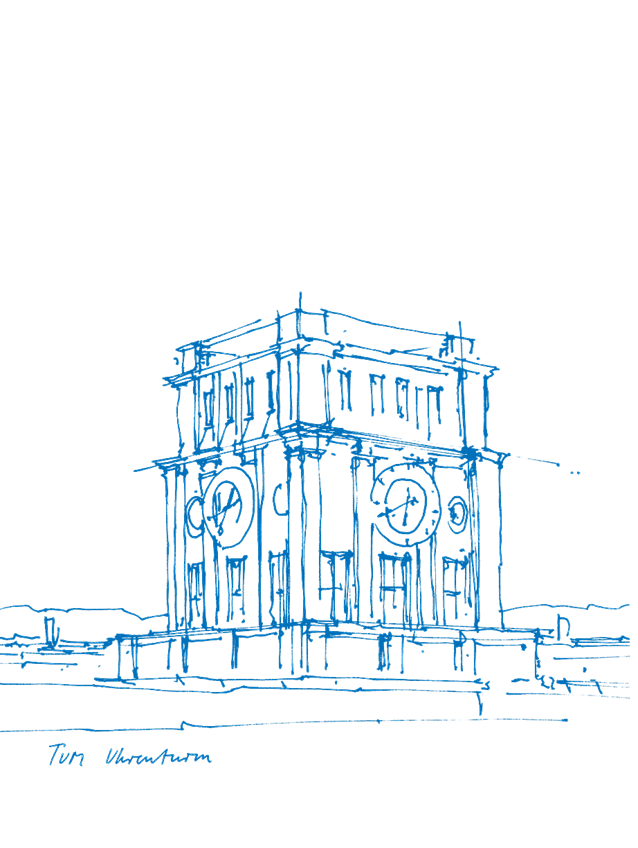
\includegraphics{./Ressources/Presentation/Images/TUM_Uhrenturm.png}%
    \end{textblock*}%
}

\newcommand{\PraesentationStartseiteUhrenturm}{%
    \setbeamertemplate{title page}{%
        \PraesentationSeitenkopfInhalt{./Ressources/_Images/Universitaet_Logo_RGB.pdf}%
        \PraesentationBildUhrenturm%
        \PraesentationTitelseiteInhalt%
    }%
}

\newcommand{\PraesentationStartseiteFlaggen}{%
    \setbeamertemplate{title page}{%
        \begin{textblock*}{\paperwidth}[0,1](-\PraesentationSeitenrand,\paperheight-\PraesentationSeitenrand)%
            
\includegraphics[min width=\paperwidth,max width=\paperheight,min totalsize={\paperwidth}{\paperheight},keepaspectratio,center]{./Ressources/Presentation/Images/Universitaet_Flaggen.jpg}%
        \end{textblock*}%
        \PraesentationSeitenkopfInhalt{./Ressources/_Images/Universitaet_Logo_weiss.pdf}%
        \PraesentationTitelseiteInhalt%
    }%
}

\newcommand{\PraesentationStartseiteLeer}{%
    \setbeamertemplate{title page}{%
        \PraesentationSeitenkopfInhalt{./Ressources/_Images/Universitaet_Logo_weiss.pdf}%
        \PraesentationTitelseiteInhalt%
    }%
}


\newcommand{\PraesentationMasterStandard}{%
    \PraesentationFarbschemaStandard%
    \PraesentationStartseiteUhrenturm%
    \setbeamertemplate{headline}{%
        \PraesentationSeitenkopfInhalt{./Ressources/_Images/Universitaet_Logo_RGB.pdf}%
    }%
}

\newcommand{\PraesentationMasterWeissBlau}{%
    \PraesentationFarbschemaWeissBlau%
    \PraesentationStartseiteLeer%
    \setbeamertemplate{headline}{%
        \PraesentationSeitenkopfInhalt{./Ressources/_Images/Universitaet_Logo_weiss.pdf}%
    }%
}


\newcommand{\PraesentationMasterKopfzeileDreizeiler}{%
    \PraesentationFarbschemaStandard%
    \setbeamertemplate{title page}{%
        \begin{textblock*}{\paperwidth}[0,0](0cm, -7.8mm)%
            \color{TUMBlau}\PraesentationSchriftgroesseDreizeiler\selectfont%
            \LehrstuhlName\\%
            \FakultaetName\\%
            \UniversitaetName\vskip0pt%
            \normalcolor\normalsize\selectfont%
        \end{textblock*}%
        \PraesentationSeitenkopfInhalt{./Ressources/_Images/Universitaet_Logo_RGB.pdf}%
        \PraesentationBildUhrenturm%
        \PraesentationTitelseiteInhalt%
    }%
    \setbeamertemplate{headline}{%
        \begin{textblock*}{\paperwidth}[0,0](0cm, 0cm)%
            \begin{minipage}[t][2cm][t]{\paperwidth}%
                \color{TUMBlau}\PraesentationSchriftgroesseDreizeiler\selectfont%
                \LehrstuhlName\\[1.38mm]%
                \FakultaetName\\[1.44mm]%
                \UniversitaetName\vskip0pt%
                \normalcolor\normalsize\selectfont%
            \end{minipage}%
        \end{textblock*}%
        \PraesentationSeitenkopfInhalt{./Ressources/_Images/Universitaet_Logo_RGB.pdf}%
    }%
}

\newcommand{\PraesentationMasterWeissSchwarz}{%
    \PraesentationFarbschemaWeissSchwarz%
    \setbeamertemplate{title page}{%
        \PraesentationTitelseiteInhalt%
        \PraesentationSeitenkopfInhalt{./Ressources/_Images/Universitaet_Logo_weiss.pdf}%
    }
    \setbeamertemplate{headline}{%
        \PraesentationSeitenkopfInhalt{./Ressources/_Images/Universitaet_Logo_weiss.pdf}%
    }
}

\newcommand{\PraesentationTitelseite}{\frame[plain]{\titlepage}}
\newcommand{\PraesentationUeberschriftZweizeilig}[2]{\frametitle{#1\\[8mm]#2}}

\setbeamersize{
    text margin left=\PraesentationSeitenrand,
    text margin right=\PraesentationSeitenrand
}

\setbeamertemplate{frametitle}{%
    {\rule{0pt}{42mm + \PraesentationPositionKorrekturOben}\PraesentationSchriftgroesseSehrGross\selectfont\insertframetitle\newline\vspace*{-6.7mm}}%
}


% Aufzählungen:
\newcommand{\PraesentationAufzaehlungEbeneEinsSymbol}{\raise2pt\hbox{\donotcoloroutermaths\usebeamercolor{itemize subitem}\PraesentationSchriftgroesseAufzaehlungszeichen$\bullet$}}
\newcommand{\PraesentationAufzaehlungEbeneZweiSymbol}{\raise1.25pt\hbox{\donotcoloroutermaths\usebeamercolor{itemize subitem}$-$}}
\setbeamertemplate{itemize items}[circle]
\setbeamertemplate{itemize subitem}[triangle]
\setbeamercolor{itemize subitem}{fg=black}
\setbeamerfont{itemize/enumerate subbody}{size=\normalsize}
\setbeamertemplate{itemize item}{\PraesentationAufzaehlungEbeneEinsSymbol}
\setbeamertemplate{itemize subitem}{\PraesentationAufzaehlungEbeneZweiSymbol{}}
%\addtolength{\leftmarginii}{16mm-2pt}%

\newenvironment{PraesentationAufzaehlung}
{%
    \vspace{-\baselineskip}%
    \begin{itemize}%
        \setlength{\itemsep}{0pt}%
        \setlength{\parskip}{0pt}%
        \setlength{\parsep}{0pt}%
        \addtolength{\itemindent}{-1ex}%
}{%
    \end{itemize}%
}


\newcommand\Warning{%
	\makebox[1.4em][c]{%
		\makebox[0pt][c]{\raisebox{.1em}{\small!}}%
		\makebox[0pt][c]{\color{TUMOrange}\Large$\bigtriangleup$}}}%

%%%%%%%%%%%%%%%%%%%%%%%%%%%%%%%%%%%%%%%%%%%%%%%%%%%%%%%%%%%%%%%%%%%%%%%%%%%%%%%%
% DOKUMENT
%%%%%%%%%%%%%%%%%%%%%%%%%%%%%%%%%%%%%%%%%%%%%%%%%%%%%%%%%%%%%%%%%%%%%%%%%%%%%%%%


% PDF-Einstellungen:
\hypersetup{
    pdfstartview={Fit},
    pdfproducer={\AllgemeinErsteller},
    pdfcreator={\AllgemeinGestalter}
}

\textblockorigin{\PraesentationSeitenrand}{\PraesentationSeitenrand} % Ursprung für Positionierung

\setbeamerfont{footnote}{size=\PraesentationSchriftgroesseKlein}

\setbeamertemplate{footline}{
    \hbox{%
        \usebeamerfont{footnote}%
        \begin{beamercolorbox}[wd=.9\paperwidth]{}%
            \hspace*{\PraesentationSeitenrand}%
            \PersonTitel{} \PersonVorname~\PersonNachname~(\UniversitaetAbkuerzung) \PraesentationFusszeileZusatz{}%
        \end{beamercolorbox}%
        \begin{beamercolorbox}[wd=.1\paperwidth]{}%
            \insertframenumber{}%
            \raggedleft
            \hspace*{\PraesentationSeitenrand}%
        \end{beamercolorbox}%
        \vspace*{3.25mm}%
    }%
}

\setbeamertemplate{navigation symbols}{}

\begin{document}
\setlength{\baselineskip}{\PraesentationAbstandAbsatz}
\setlength{\parskip}{\baselineskip}
\lstset{language=C++,
		basicstyle=\ttfamily,
		keywordstyle=\color{TUMBlau}\ttfamily,
		stringstyle=\color{TUMOrange}\ttfamily,
		commentstyle=\color{TUMGruen}\ttfamily,
		morecomment=[l][\color{magenta}]{\#},
		aboveskip=0.5\medskipamount,
		belowskip=0.5\medskipamount,
		frame = single,
		numbers=left,
		stepnumber=1,
		escapeinside={(*@}{@*)}
	}
 
%%%%%%%%%%%%%%%%%%%%%%%%%%%%%%%%%%%%%%%%%%%%%%%%%%%%%%%%%%%%%%%%%%%%%%%%%%%%%%%%



%%%%%%%%%%%%%%%%%%%%%%%%%%%%%%%%%%%%%%%%%%%%%%%%%%%%%%%%%%%%%%%%%%%%%%%%%%%%%%%%
% FOLIENSTIL: Standard
% !!!ÄNDERUNG HIER:!!!
\PraesentationMasterStandard
%\PraesentationMasterKopfzeileDreizeiler
%\PraesentationMasterWeissBlau

%\PraesentationStartseiteFlaggen
\PraesentationStartseiteUhrenturm
\PraesentationTitelseite % Fügt die Startseite ein

\begin{frame}
	\frametitle{Overview}
	\vspace{1cm}
	\begin{minipage}[s]{\textwidth}
	\tableofcontents
	\end{minipage}
\end{frame}

\section{Union-Find}
\begin{frame}
\frametitle{Union-Find}
\begin{itemize}
	\item Models a partial equivalence relation
over a finite domain
	\item Implemented by disjoint set forests
\item The graph structure is represented by an array
	\item Supports \textbf{Union} and \textbf{Find} operations
\end{itemize}
\vspace{-2cm}
\begin{figure}
	\centering
	\begin{minipage}{5cm}
		\caption{Two equivalence classes}\end{minipage}
	\begin{minipage}{8cm}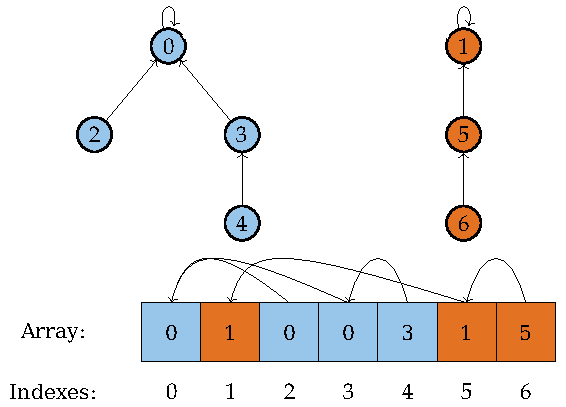
\includegraphics[scale=1.0]{UnionFindFigure}\end{minipage}
\end{figure}
\end{frame}

\subsection{Path Compression and Union by Rank}
\begin{frame}
\frametitle{Path Compression and Union by Rank}
\begin{itemize}
	\item As with many tree-based data structures, trees should be kept flat
	\item This is done in two ways: 
	\begin{enumerate}
		\item \textbf{Path Compression}
		\item \textbf{Union by Rank}
	\end{enumerate}
\end{itemize}	
\begin{figure}
	\centering
	\begin{minipage}{5cm}
		\caption{Illustration of Path Compression}\end{minipage}
	\begin{minipage}{8cm}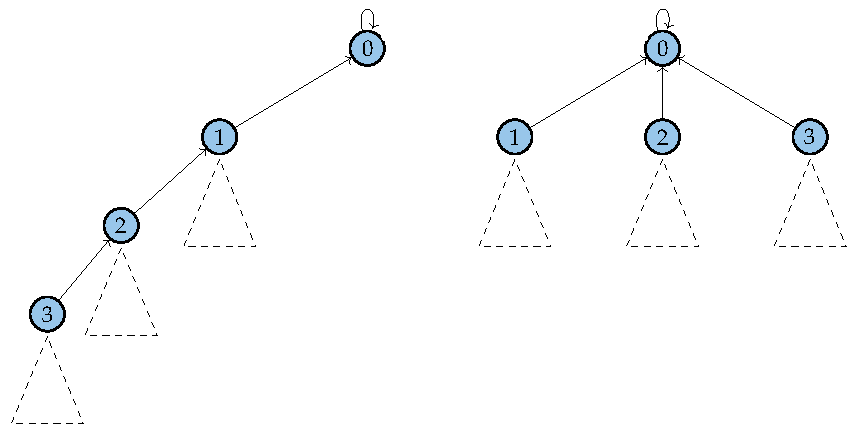
\includegraphics[scale=0.8]{PathCompressionFigure}\end{minipage}
\end{figure}
\end{frame}

\subsection{Design Choices}
\begin{frame}
	\frametitle{Design Choices}
	\begin{itemize}
		\item Done in Imperative/HOL, which can then be exported to several languages
		\item The arrays used and therefore the domain are static
		\item We define the operations in Imperative/HOL:
		\begin{itemize}
			\item 
\includegraphics{RepofDef}
			\item 
\includegraphics{CompressDef}
			\item 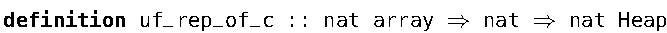
\includegraphics{RepofcDef}
			\item 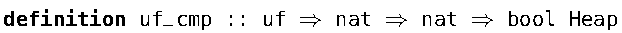
\includegraphics{CmpDef}
			\item 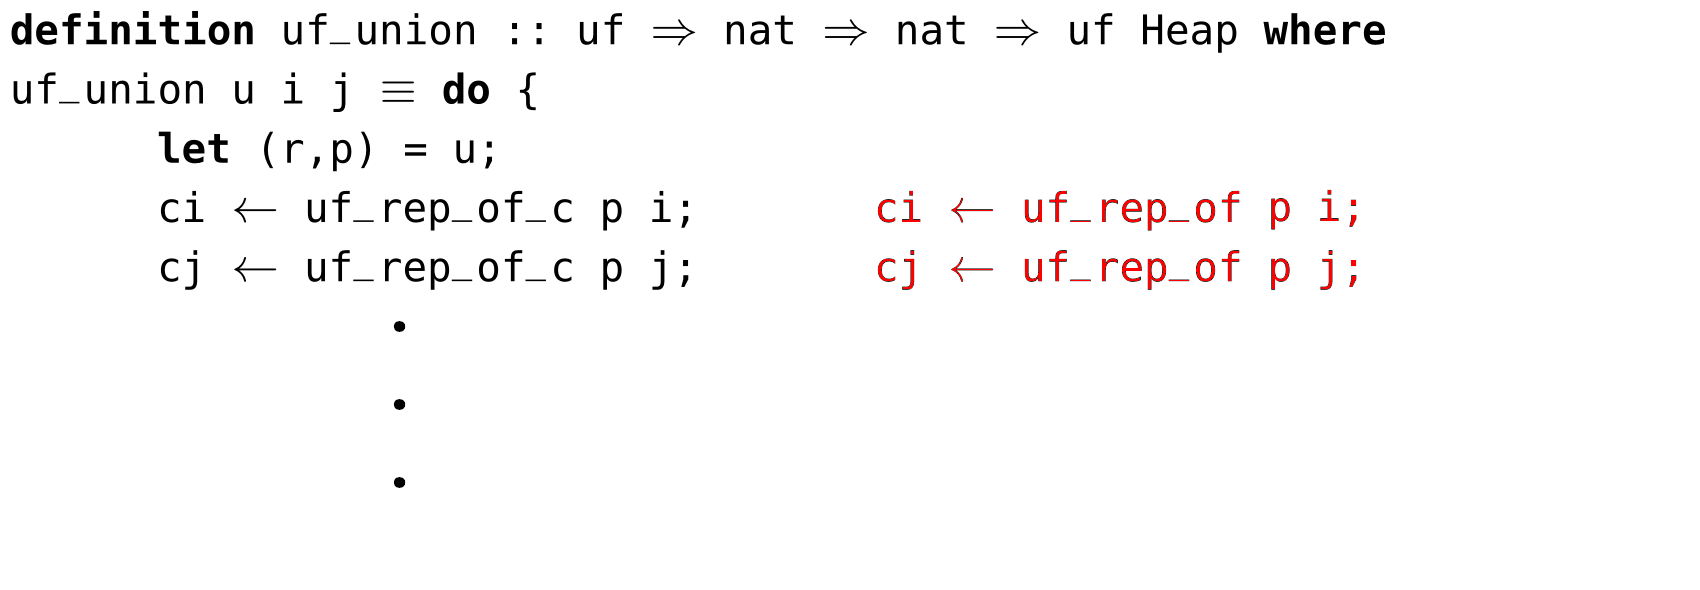
\includegraphics{UnionBigDef.png}
		\end{itemize}
	\end{itemize}
\end{frame}

\section{History of the Proof}
\begin{frame}
	\frametitle{History of the Proof}
	\begin{itemize}
		\item Several, slightly different results about the amortized time complexity of the operations of Union-Find
		\item The first result involving $\alpha$ by Tarjan in 1975. The proof was simplified until the version in CLRS
		\item In 1989 Fredman and Saks prove (in some sense) the optimality of the result
		\item The latest result by Alstrup et al. in 2014 tightens the bound
		\item In 2017, Charguéraud and Pottier formalize the result in Coq
		\item Now, we present this formalization in Isabelle/HOL
		\item In all these proofs, but especially since Alstrup et al., most work is needed for the abstract analysis
	\end{itemize}
\end{frame}

\section{Timeline of the Project}
\begin{frame}
	\frametitle{Timeline of the Project}
	\vspace{-0.7cm}
	\begin{table}
		\centering
		\begin{minipage}[t]{\linewidth}
			\color{gray}
			\ytl{May}{Background work: Familiarisation with Sepreftime and the paper by Charguéraud and Pottier}
			\vspace{-0.1cm}
			\ytl{May 15th}{Official thesis registration}
			\vspace{-0.1cm}
			\ytl{June}{Cleanup of the previous work by Lammich and Haslbeck}
			\vspace{-0.1cm}
			\ytl{June 5th}{Armaël Guéneau visits TUM}
			\vspace{-0.1cm}
			\ytl{June}{\textbf{Bottom-up}: Ackermann and InverseNatNat theories and important definitions}
			\vspace{-0.1cm}
			\ytl{July}{First abstract proofs: rank, level, index}
			\vspace{-0.1cm}
			\ytl{July 16th}{\textbf{Top-down}: Sanity check of definitions done, skipping the rest and proof of the Hoare-Triples}
			\vspace{-0.1cm}
			\ytl{August}{Exam phase}
			\vspace{-0.1cm}
			\ytl{September}{Parallel writing of the thesis, proof gap-filling and correction of definitions}
			\vspace{-0.1cm}
			\ytl{September 8th}{Complete sound theory}
			\vspace{-0.1cm}
			\ytl{Semptember 13th}{Submission of the thesis}
			\vspace{-0.1cm}
			\bigskip
		\end{minipage}%
	\end{table}
\end{frame}

\section{Overview of the Isabelle Proof}
\begin{frame}
	\frametitle{Overview}
	\vspace{-2.5cm}
	\begin{figure}
		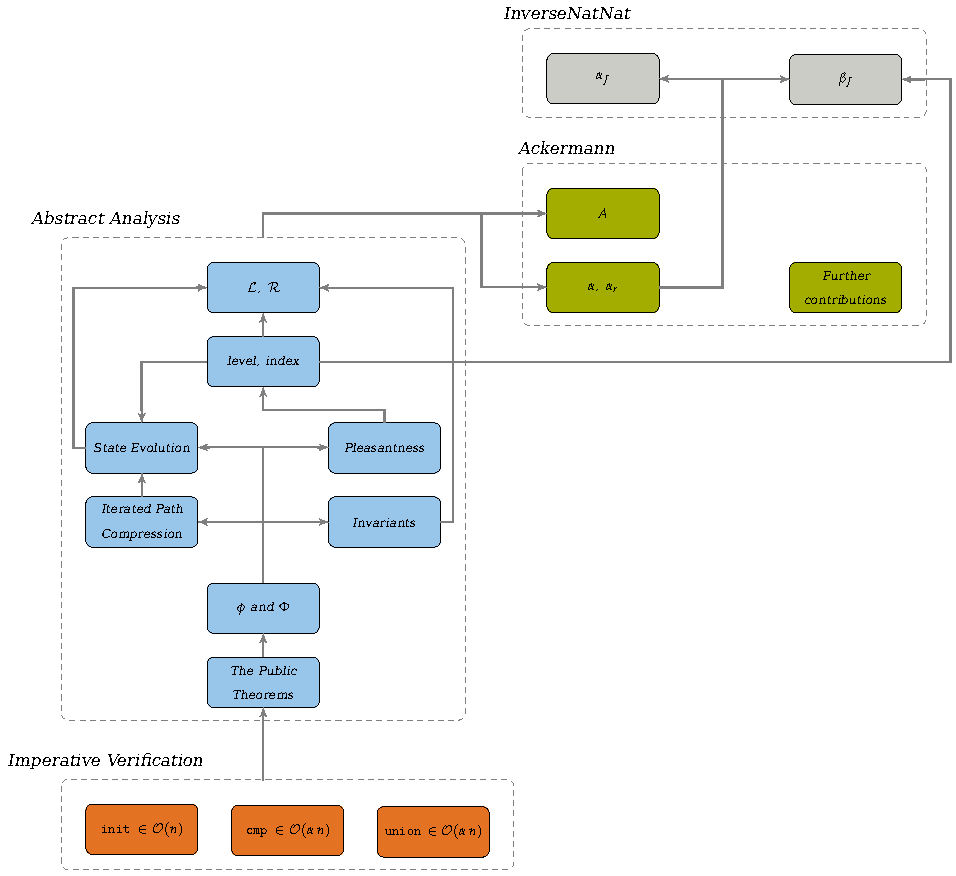
\includegraphics[scale=0.8]{OverviewFigure}
	\end{figure}
\end{frame}

\section{Inverses of Functions $f: \mathbb{N} \rightarrow \mathbb{N}$}
\begin{frame}
	\frametitle{Inverses of Functions $f: \mathbb{N} \rightarrow \mathbb{N}$}
	\begin{minipage}[t]{0.55\linewidth}
		\vspace{-4cm}
	\begin{itemize}
		\item Defined in InverseNatNat.thy
		\item Upper inverse $\alpha_f$ and Lower inverse $\beta_f$
		\item Lemmas to change the proof obligations between inverses and the original function
		\item Used for Inverse Ackermann Function, but also the ``index'' of a node
	\end{itemize}
	\end{minipage}
\begin{minipage}[c]{0.4\linewidth}
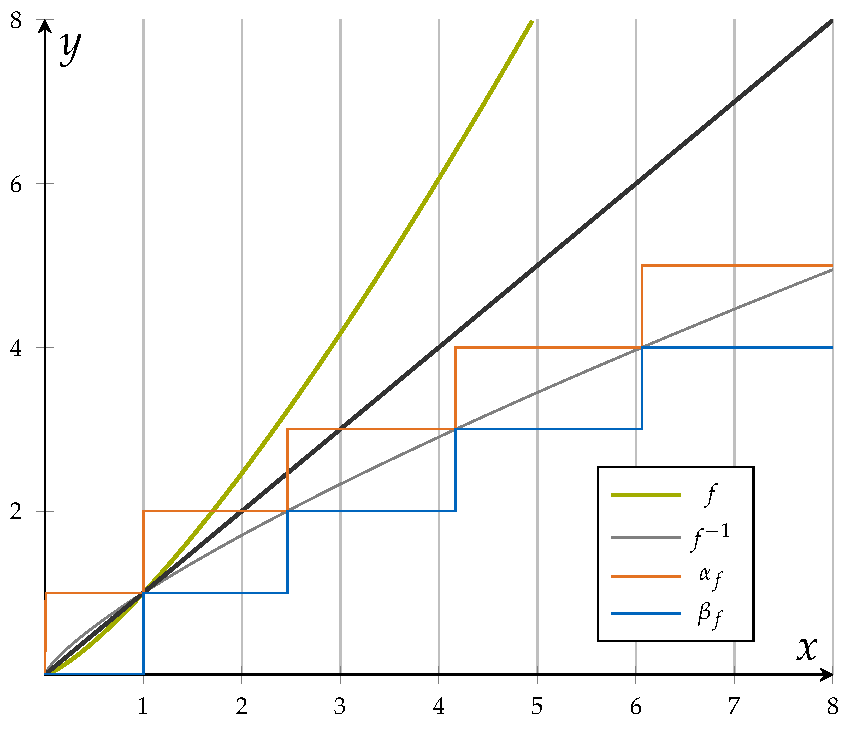
\includegraphics[scale=0.7]{InverseNatNatFigure}
\end{minipage}
\end{frame}

\section{The Ackermann Function and its Inverse}
\begin{frame}
	\frametitle{The Ackermann Function and its Inverse}
	\begin{itemize}
		\item There is no single Ackermann Function ``$A$'' or inverse Ackermann Function ``$\alpha$''
		\item All definitions share the property of growing faster than any primitive recursive function
		\item $\alpha$ grows \textbf{very} slowly
		\item We use the definition of $A$ and $\alpha$ by Tarjan:
	\end{itemize}
\begin{minipage}{0.45\linewidth}
\begin{dfn} Ackermann Function
	\begin{align*}
	A \, 0 \, x &= x + 1  \\
	A \, (k + 1)\, x &= (A\, k)^{(x + 1)}\, x 
	\end{align*}
\end{dfn}
\end{minipage}
\begin{minipage}{0.45\linewidth}
\begin{dfn} Inverse Ackermann Function
	\begin{align*}
	\alpha \, n &= \min \{ k \,\mid\, A\, k\, 1 \geq n \}\\
	\alpha_r \, n &= 1 + \min\{ k \,\mid\, A\, k\, r \geq (n + 1) \}
	\end{align*}
\end{dfn}
\end{minipage}

\begin{itemize}
	\item In Isabelle/HOL, the definitions are expressed slightly differently and make use of InverseNatNat.thy
\end{itemize}
\end{frame}

\begin{frame}
	\frametitle{The Ackermann Function and its Inverse}
	\vspace{0.6cm}
	\begin{lma}{observable\_universe\_$\alpha$}
		\newline
		\textbf{Assume:} $n \leq 10^{80} $
		\begin{equation}
		\alpha \, n \leq 4 \label{universealpha}
		\end{equation}
	\end{lma}	
\begin{itemize}
	\item $10^{80}$ is an estimate of the number of atoms in the universe
\end{itemize}

\begin{lma}{$\alpha$\_n\_0\_$\alpha$\_logn}
	\newline
	\textbf{Assume:} $16 \leq n$
	\begin{equation}
	\alpha \, n \leq 1 + (\alpha \, (\log{n}))
	\end{equation}
\end{lma}
\begin{itemize}
	\item $\alpha$ and $\alpha(\log\, n)$ are asymptotically equivalent
	\item True for every primitive recursive strictly monotonic function
\end{itemize}
\end{frame}

\section{Separation Logic with Time Credits}
\begin{frame}
	\frametitle{Separation Logic with Time Credits}
	\begin{itemize}
		\item Logic to reason about mutable resources in a heap. Enables Hoare-Triple definition
		\item It also allows for ``pure'' assertions, predicates independent of the heap content
		\item Time Credits can also appear in assertions and are required to execute atomic operations
		\item The components of the logic are: \begin{itemize}
			\item $\uparrow(P)$ 
			\item true and false 
			\item $p \mapsto_a xs$ 
			\item $P_1 * P_2$ 
			\item $\exists_A x.\, P$ 
		\end{itemize}
	\item The Framework by Haslbeck implementing this for Isabelle/HOL, as well as this thesis as a usage example will be published in the AFP.
	\end{itemize}
\end{frame}

\subsection{Amortized Analysis with Time Credits}
\begin{frame}
	\frametitle{Amortized Analysis with Time Credits}
	\begin{itemize}
		\item We define a potential function $\Phi$ that measures the ``entropy'' of the data structure
		\item The idea is to ``hide'' $\Phi$ credits in the assertion defining the data structure
		\item If we are able to prove a Hoare-Triple of the form:
		\begin{equation*}
		\langle \mathrm{invar}(\mathcal{D}) * \$(\Phi(\mathcal{D})) * \underbrace{\$(f(\mathcal{D}))}_{\text{Advertised Cost}} \rangle 
		\quad \mathtt{op}(\mathcal{D}) \quad 
		\langle \mathrm{invar}(\mathcal{D'}) * \$(\Phi(\mathcal{D}')) \rangle
		\end{equation*}
		for any $\Phi$ and $f \in \mathcal{O}(g)$, we can conclude that the operation \texttt{op} has an amortized cost in $\mathcal{O}(g)$
		\item Remaining questions: \begin{itemize}
			\item What $\Phi$ do you choose? How does $\Phi$ evolve?
			\item How do you prove the functional correctness? \newline
			$\Longrightarrow$ Mathematical analysis of the data structure
		\end{itemize}
	\end{itemize}
\end{frame}


\section{The Potential Function $\Phi$}
\begin{frame}
	\frametitle{The Potential Function $\Phi$}	
	\vspace{0.6cm}
	\begin{definition}{Potential for a single node}
		\begin{equation*}
		\philr i :=
		\begin{cases}
		\alpha_r\, (\RR_r\, i) \cdot (1 + (\RR_r\, i)) & \mathrm{if}\, \LL!i=i \,   \\
		(\alpha_r\, (\RR_r\, i) - \level i) \cdot \RR_r\, i - \iindex i + 1  &\mathrm{if}\, \alpha_r\, (\RR_r\, i) = \alpha_r\, (\RR_r\, (\LL!i))\\
		0 & \mathrm{otherwise}
		\end{cases}
		\end{equation*}
	\end{definition}

\begin{definition}{Potential of the data structure}
	\begin{equation}
	\Philr :=  \sum_{i = 0}^{|\LL| - 1}{\philr i}
	\end{equation}
\end{definition}

\begin{itemize}
	\item $\{0,\dots, |\LL|-1\}$ is in this case the domain of our equivalence relation
\end{itemize}

	
\end{frame}


\section{Results of the Thesis}
\begin{frame}
	\frametitle{Results of the Thesis}
	The $\,\,\mathrm{is\_uf}$ Assertion takes a relation and two arrays as arguments and ensures:\begin{itemize}
		\item The well-formedness of the disjoint set forest and the ranks
		\item That the relation modeled by the array is the one given
		\item That the necessary potential is stored as Time Credits
	\end{itemize}
	\vspace{0.6cm}
	\begin{dfn}
	\begin{align}
	\begin{split}
	\mathrm{is\_uf}\, \mathcal{X} \, (s,p) := 
	&\exists_A \LL\, \RR.\, p \mapsto_a \LL * s \mapsto_a \RR\, * \\
	&\uparrow (\ufaalpha = \mathcal{X} \land \mathrm{invar\_rank}\, \LL \, \RR)\, * \\
	&\$(4\cdot\Philr)
	\end{split}
	\end{align}
	\end{dfn}
\vspace{-0.5cm}
\end{frame}

\begin{frame}
	\frametitle{Results of the Thesis}
	\vspace{0.6cm}
	\begin{minipage}{0.48\linewidth}
\begin{lma}
	\begin{equation*}
	\mathrm{uf\_cmp\_time}\, \in \mathcal{O}(\alpha_r\,n)
	\end{equation*}
\end{lma}

\begin{thm}
	\,\newline
	\begin{align*}
	\begin{split}
	\langle \mathrm{is\_uf}\, \mathcal{X}\, u\, * &\$(\mathrm{uf\_cmp\_time}\, |\mathrm{Dom}\, \mathcal{X}|)\rangle \quad \\ 
	&\mathtt{uf\_cmp}\, u\, i\, j\\
	&\langle \mathrm{is\_uf}\, \mathcal{X}\, u\, * \uparrow(r \leftrightarrow (i,j)\in\mathcal{X}) \rangle_t
	\end{split}
	\end{align*}
\end{thm}
	\end{minipage}
	\begin{minipage}{0.40\linewidth}
\begin{lma}
	\begin{equation*}
	\mathrm{uf\_union\_time}\, \in \mathcal{O}(\alpha_r\,n)
	\end{equation*}
\end{lma}
\begin{thm}\,\newline
	\textbf{Assumes: } $i,j \in \mathrm{Dom}\, \mathcal{R}$
	\begin{align*}
	\begin{split}
	\langle \mathrm{is\_uf}\, \mathcal{X}\, u\, * &\$(\mathrm{uf\_union\_time}\, |\mathrm{Dom}\, \mathcal{X}|)\rangle \quad \\
	&\mathtt{uf\_union}\, u\, i\, j\\
	&\langle \mathrm{is\_uf}\, (\mathrm{per\_union}\, \mathcal{X}\, i\, j)\rangle_t
	\end{split}
	\end{align*}
\end{thm}
\end{minipage}
\vspace{-0.4cm}
\begin{itemize}
	\item \texttt{uf\_union} corresponds to the \textbf{Union} and \texttt{uf\_cmp} to the \textbf{Find} operation
	\item These theorems follow from abstract results about disjoint set forests
	\item The whole proof is about 5KLoc long in Isabelle/HOL
\end{itemize}
\end{frame}

\section{Conclusions}
\begin{frame}
	\frametitle{Conclusions}
	\begin{itemize}
		\item Formalization of the state-of-the-art result about Union-Find
		\item Comprehensive theory about Ackermann, including quantitative and asymptotic results
		\item The proofs of the imperative programs are still too long:
		 \begin{itemize}
			\item The automation does not deal well with arithmetic
			\item It also instantiates existentials too aggressively
			\item Repetitive proofs generated by branching $\Longrightarrow$ optimization possible
		\end{itemize}
		\item Formal verification of non-trivial results about runtime, not only correctness are possible 
		\item Some overhead, but this helps to reveal hidden assumptions 
	\end{itemize}
\end{frame}

%\PraesentationMasterKopfzeileDreizeiler
\begin{frame}
\frametitle{\,}
\Huge Thank You for listening! \newline
\Huge Any questions?
\end{frame}

\begin{frame}
	\frametitle{Important Definitions}
	\vspace{1cm}
	\begin{definition}{invar\_rank}
		\begin{align}
		\mathrm{invar\_rank}\, \LL \, \RR := 
		&\mathrm{ufa\_invar} \, \LL \, \land \\
		&|\LL| = |\RR| \, \land \\
		&(\forall (i,j) \in \ufabstart. \, \RR!i < \RR!j) \\
		&(\forall i < |\LL|.\, \LL!i = i \longrightarrow 2^{\RR!i} \leq |\mathrm{descendants}_\LL \, i|)
		\end{align}
	\end{definition}
	\begin{definition}{ufa\_invar}
	\begin{equation}
	\mathrm{ufa\_invar} \, \LL \, := \forall i < |\LL|.\, i \in \mathrm{Dom}\, \repof \land \LL!i < |\LL|
	\end{equation}
	\end{definition}

\begin{definition}{ufa\_$\beta$\_start}
\begin{equation}
\ufabstart := \{(x,y) \,\mid\, x<|\LL| \land y<|\LL| \land x \neq y \land \LL!x = y \}
\end{equation}
\end{definition}

\end{frame}



%%%%%%%%%%%%%%%%%%%%%%%%%%%%%%%%%%%%%%%%%%%%%%%%%%%%%%%%%%%%%%%%%%%%%%%%%%%%%%%%
\end{document} % !!! NICHT ENTFERNEN !!!
%%%%%%%%%%%%%%%%%%%%%%%%%%%%%%%%%%%%%%%%%%%%%%%%%%%%%%%%%%%%%%%%%%%%%%%%%%%%%%%%
